\section{Auswertung}

\subsection{Stationäres Verhalten}

Um die Kennlinienfelder zu erstellen werden die Messwerte aus \autoref{tab:M1_12_werte} in Matlab übernommen und als Punkte geplottet. Anschließend wird für jeden Parameterwert eine Ausgleichsgerade geplotttet. Davon ausgehend, dass die Heiz- und Lüfterleistung proportional zum jeweiligen Sollwert sind, kann mit diesen Kennlinienfelder eine Aussage getroffen werden, auf welche Temperatur sich die Regelstrecke bei bestimmten einstellt.

Das Kennlinienfeld für variablen Heizungssollwert und konstanten Lüftersollwert als Parameter ist in \autoref{fig:A1_1_kennlinienfeld} abgebildet. Das Kennlinienfeld für variablen Lüftersollwert und konstanten Heizungssollwert als Parameter ist in \autoref{fig:A1_2_kennlinienfeld} abgebildet.

\begin{figure}[h]
    \begin{center}
        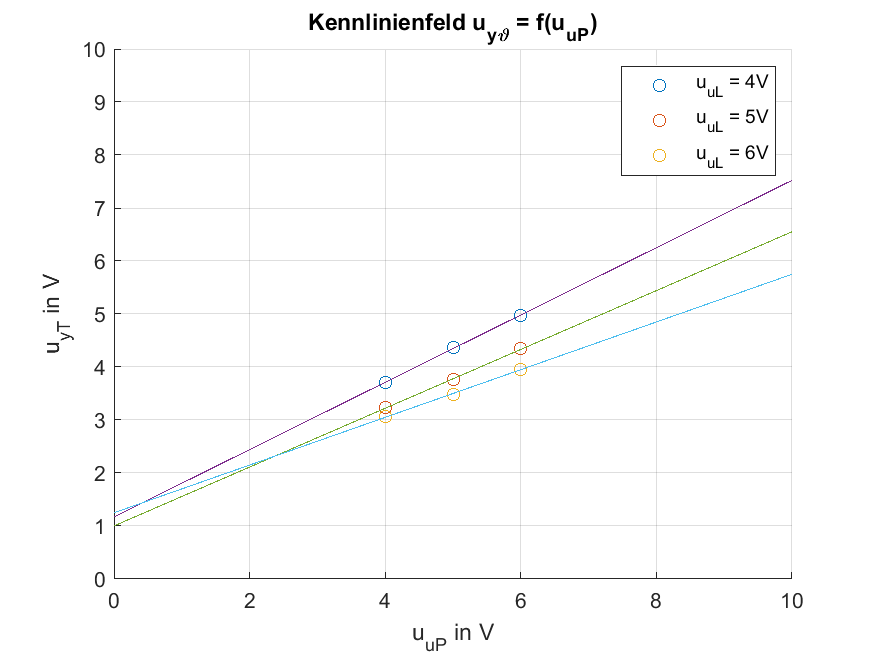
\includegraphics[width=0.8\textwidth]{img/A1_1.png}
        \caption{Kennlinienfeld \( U_{y\vartheta} = f\left(U_{uP}\right) \)}
        \label{fig:A1_1_kennlinienfeld}
    \end{center}
\end{figure}

\newpage

\begin{figure}[h]
    \begin{center}
        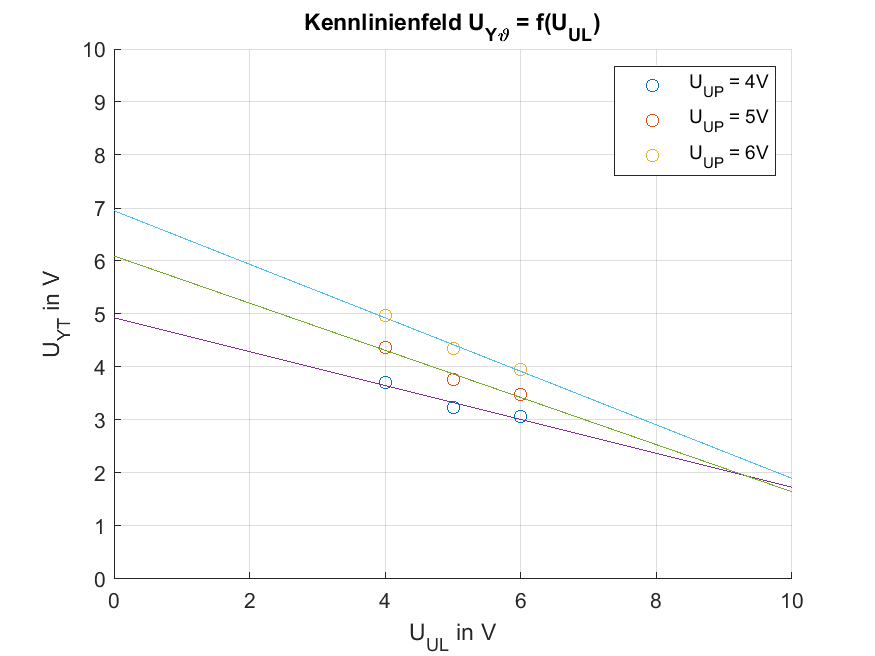
\includegraphics[width=0.8\textwidth]{img/A1_2.png}
        \caption{Kennlinienfeld \( U_{y\vartheta} = f\left(U_{uL}\right) \)}
        \label{fig:A1_2_kennlinienfeld}
    \end{center}
\end{figure}

\subsubsection{A1.4: Lineare Interpolation}

Verwendet man für die Ausgleichsgerade die etwas ungenauere Formel \( y = m\cdot x \), erhält man aus der numerischen Berechnung den Parameter  \( m = \SI{0.7501}{} \), Dies ist dementsprechend die Streckenverstärkung:

\[K_{ges} = \frac{\Delta u_{y\theta}}{\Delta u_{uP}} = K_u \cdot K_S \cdot K_M = \SI{0.7501}{} \]

Weiterhin gilt:

\[K_S = \frac{\Delta \theta}{\Delta P_{el}} ; K_u = \frac{\Delta P_{el}}{\Delta u_{uP}} ; K_M = \frac{\Delta u_{y\theta}}{\Delta \theta}\]


Um die Werte für \( U_{y\vartheta} \) und \( U_{uP} \) bei der gegeben Temperatur \( \vartheta = \SI{46}{\celsius} \) auszurechnen, wird zunächst die Steigung einer Ausgleichsgerade für das Verhältnis zwischen Temperatur und Ausgangsspannung des Temperatursensors numerisch berechnet. Anschließend lassen sich die Spannungswerte berechnen:

\[ U_{y\vartheta} = f\left(\vartheta\right) = \frac{\vartheta}{\SI{10.9512}{\celsius\per\volt}} = \frac{\SI{46}{\celsius}}{\SI{10.9512}{\celsius\per\volt}} = \SI{4,2}{\volt} \]
\[ U_{uP} = \frac{U_{y\vartheta}}{K_S} = \frac{\SI{4,2}{\volt}}{\SI{0.7501}{}} = \SI{5,599}{\volt} \]

\newpage


\subsection{Dynamisches Verhalten}

Um das dynamische Verhalten der Regelstrecke abzubilden, soll als Modell ein PT1-Glied mit Totzeit verwendet werden.  Das Modell lässt sich durch folgende Formel beschreiben:

\[ G_S\left(s\right) = \frac{\vartheta\left(s\right)}{P_{el}\left(s\right)} = K_S \frac{e^{-T_t s}}{1+T_S s}\]

Um die Parameter zu bestimmen, werden die Messwert zunächst in Matlab geladen und der Zeitindex des Sprungs manuell bestimmt. Anschließend wird der Mittelwert des Heizungs-Stellgrades jeweils vor und nach dem Sprung bestimmt. Der Mittelwert vor dem Sprung wird elementweise von dem gesamten Datensatz abgezogen, um den Offset auf null zu setzen. Der Mittelwert nach dem Sprung wird für die Berechnung der Proportionalverstärkung des System benötigt. Vom dem Temperatur-Istwert werden ebenfalls alle Werte vor dem Sprung gemittelt und elementweise von dem Istwert-Datensatz abgezogen, ebenfalls um den Offset zu entfernen. Anschließend werden die Werte der letzten 10 Sekunden gemittelt und als Endwert angenommen. Mit dem Endwert und die mittleren Sollwert nach dem Sprung wird die Proportionalverstärkung berechnet. Anschließend wird mit diesem Wert ein das mathematische Modell der Regelstrecke gebildet. Die Parameter für die Ausgleichs- und Verzugszeit werden anschließend nur Anwendung der Methode der kleinsten Quadrate ermittelt. Dafür werden Werte in einem relativ weiten Bereich durchprobiert. Das Modell wird mit dem gemessenen Heizungs-Sollwert simuliert und anschließend die Differenz zur gemessenen Sprungantwort berechnet und ausgewertet. Die optimalen Parameter werden ausgegeben und sind in \autoref{tab:A1_6_parameter} gelistet. Die aufbereiteten Daten und die Sprungantwort des Modells sind in \autoref{fig:A1_6_a_fit} und \autoref{fig:A1_6_a_fit} als Plot dargestellt.

\begin{figure}[h]
    \begin{center}
        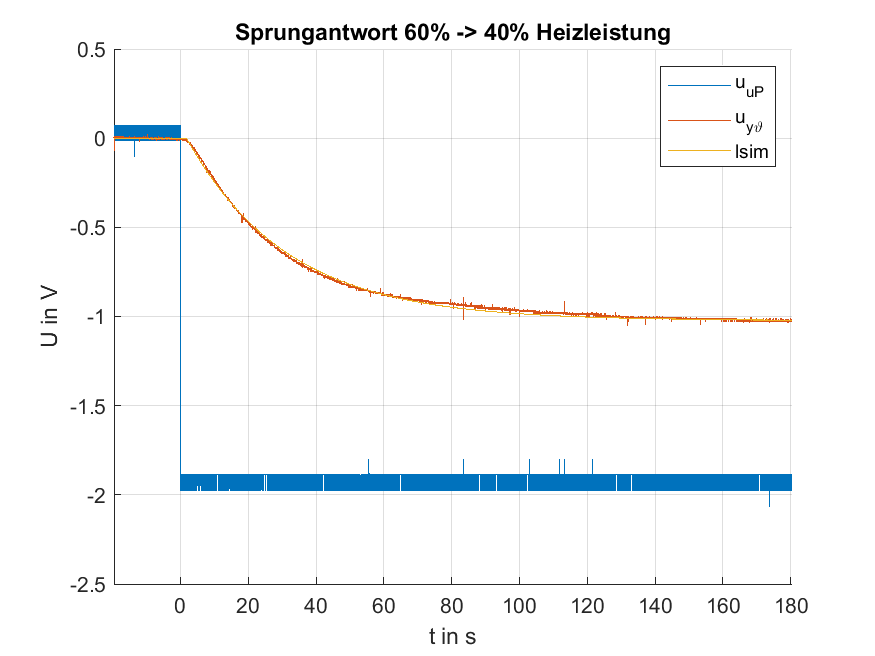
\includegraphics[width=0.8\textwidth]{img/A1_6_a.png}
        \caption{Plot der gemessen Werte und optimalem Modell für Messung 1}
        \label{fig:A1_6_a_fit}
    \end{center}
\end{figure}

\begin{figure}[h]
    \begin{center}
        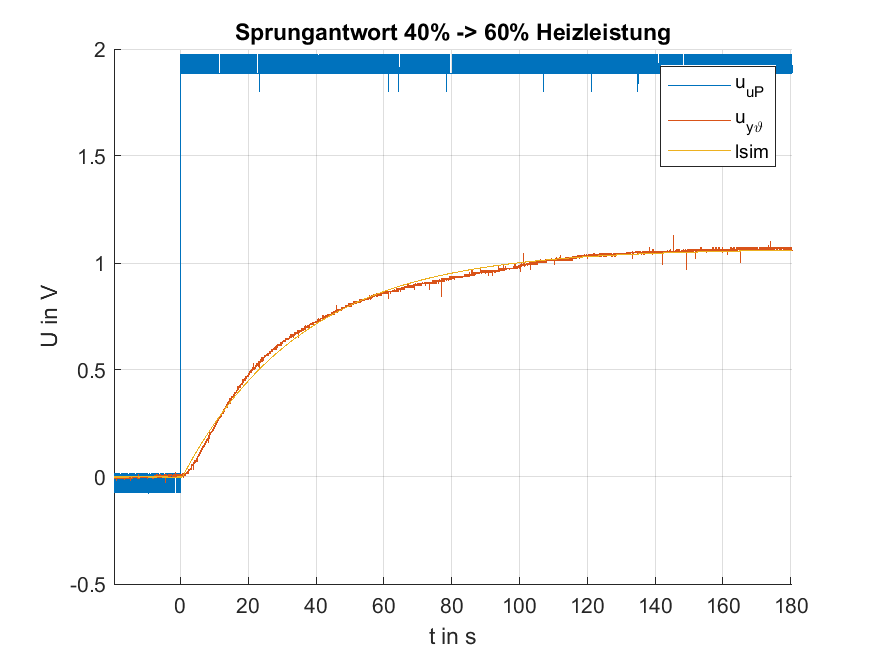
\includegraphics[width=0.8\textwidth]{img/A1_6_b.png}
        \caption{Plot der gemessen Werte und optimalem Modell für Messung 2}
        \label{fig:A1_6_a_fit}
    \end{center}
\end{figure}



\begin{table}[H]
    \begin{center}
    \begin{tabular}{|c|c|c|c|}\hline
    \tbf{Parameter} & \tbf{Messung 1}               & \tbf{Messung 2}               \\ \hline
    \( K_s \)       & \SI{0.5378}{\kelvin\per\watt} & \SI{0.5611}{\kelvin\per\watt} \\ \hline
    \( T_s \)       & \SI{29.77}{\second}           & \SI{35.52}{\second}           \\ \hline
    \( T_t \)       & \SI{1.83}{\second}            & \SI{0.58}{\second}            \\ \hline
    \end{tabular}
    \caption{Per numerischer Berechnung bestimmte optimale Parameter}
    \label{tab:A1_6_parameter}
    \end{center}
\end{table}